\documentclass{article}

\usepackage{graphicx}

% Set page margin
\usepackage[a4paper,left=1cm,right=1cm,top=1cm,bottom=2cm]{geometry}

% Set font family
\usepackage{noto}

% Set line space
\usepackage{setspace}
\onehalfspacing

% Disable para indent
\setlength{\parindent}{0pt}

% Set para space
\setlength{\parskip}{0.5\baselineskip}

% Add table support
\usepackage{booktabs}

% Add plot support
\usepackage{pgfplots}
\pgfplotsset{width=10cm,compat=1.9}

\usepackage{tikz}
\usetikzlibrary{positioning}
\usetikzlibrary{shapes.geometric}
\usetikzlibrary{shapes.multipart}

\usepackage{amsmath}

\usepackage{hyperref}

\usepackage{url}

\usepackage{float}

\usepackage{titlesec}

\usepackage{listings}

\titleformat{\section}
{\normalfont\large\bfseries}{\thesection}{1em}{}
\titlespacing*{\section}{0pt}{1ex plus 0.2ex minus 0.2ex}{0.5ex plus 0.2ex}

\begin{document}

\title{	\vspace{-1cm} \Large Group Project : Earth and Environmental Science \\ \vspace{0.2cm} \normalsize Data Integration and Visualization for the Low Burn Hall Estate - Datacube \vspace{-0.3cm}}
\author{ \normalsize Huixiaqing Liu - fhnp96}
\date{}
\maketitle

\section{Introduction}

Effective management of natural resources requires a comprehensive understanding of the target environment. This often needs the integration of data from multiple sources to characterize the site of interest.

This project aimed to develop a datacube incorporating field-collected resistivity and ground-penetrating radar (GPR) data, satellite imagery and MODIS-derived products for the Low Burn Hall Estate. The original objective was to enable interactive 3D visualization of the datacube. However, due to computational limitations, a 2D composite image has been created as a substitution.

This report details the data collection, processing and integration methodologies, presents the results, discusses the limitations and proposes future improvements.

\section{Data Collection}

\subsection{Fieldwork}

Resistivity data was collected at two locations (P1 and P2) within the estate using a resistivity meter. Measurements were taken at increasing electrode spacings to sample increasing depths.

Ground-penetrating radar (GPR) surveys were conducted using a Pulse EKKO system at positions P1 and P2. An additional GPR survey was carried out at position P1 using the wide-angle reflection and refraction (WARR) method. GPR two-way travel times were converted to depth using estimated velocities.

\begin{table}[H]
	\centering
	\begin{tabular}{cccccc}
		\hline
		Potential 1/2 Spacing & Current 1/2 Spacing & Measure 1 & Measure 2 & Measure 3 & Measure 4 \\
		\hline
		5                     & 15                  & 78.1      & 78.1      & 78.2      & 78.9      \\
		5                     & 20                  & 42        & 41.9      & 41.8      & 41.7      \\
		\hline
	\end{tabular}
	\caption{Example resistivity input data}
\end{table}

\begin{table}[H]
	\centering
	\begin{tabular}{cccccc}
		\hline
		Tool  & Interpretation & GPR Line      & Position (m) & Depth (m) & Velocity              \\
		\hline
		Point & Pink           & Lineset/line1 & 0.43         & 0.67      & Moist Soil (0.1 m/ns) \\
		Point & Pink           & Lineset/line1 & 4.03         & 3.96      & Moist Soil (0.1 m/ns) \\
		\hline
	\end{tabular}
	\caption{Example GPR interpretation input data}
\end{table}

\subsection{Provided Data}

Satellite imagery of the estate was provided as a georeferenced TIFF file.

MODIS land surface temperature (LST) and vegetation index products were provided as CSV files at a 1 km spatial resolution for 2001 and 2019.

\begin{table}[H]
	\centering
	\begin{tabular}{cccccccccc}
		\hline
		Year & Day & Easting & Northing & LST\_day & LST\_night & NDVI   & EVI    & Easting\_km & Northing\_km \\
		\hline
		2001 & 0   & 426625  & 538600   & 0        & 287.52     & 0.7755 & 0.5446 & 426         & 538          \\
		2001 & 1   & 426625  & 538600   & 300.78   & 285.94     & 0.7755 & 0.5446 & 426         & 538          \\
		\hline
	\end{tabular}
	\caption{Example MODIS input data}
\end{table}

\section{Data Processing and Integration}

\subsection{Resistivity Data}

The resistivity data was cleaned by removing negative and outlier measurements. The cleaned data was then inverted using a 6-layer model in pygimli to estimate the true resistivity structure at each location. Figure \ref{fig:res_p1} shows the raw and inverted resistivity data for Position 1, while Figure \ref{fig:res_p2} shows the same for Position 2.

\begin{figure}[H]
	\centering
	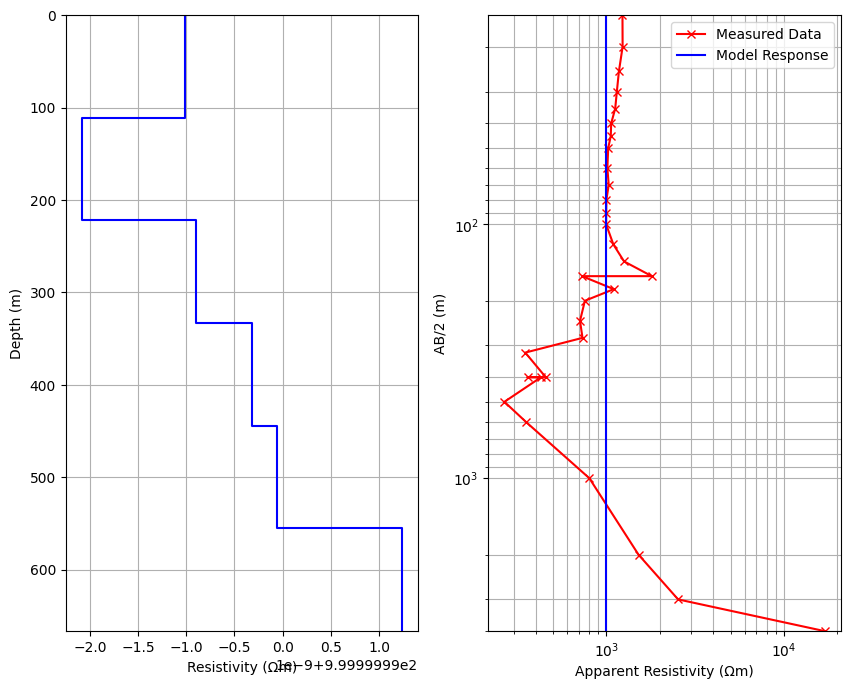
\includegraphics[width=0.8\textwidth]{resistivity_p1.png}
	\caption{Inverted and raw resistivity measurements at P1}
	\label{fig:res_p1}
\end{figure}

\begin{figure}[H]
	\centering
	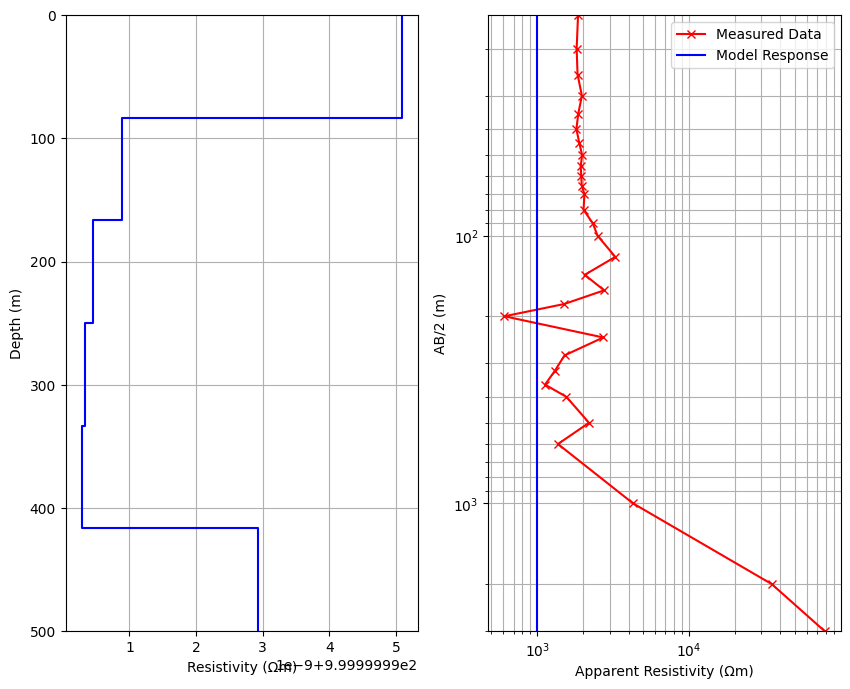
\includegraphics[width=0.8\textwidth]{resistivity_p2.png}
	\caption{Inverted and raw resistivity measurements at P1}
	\label{fig:res_p2}
\end{figure}

\subsection{GPR Data}

The raw data was stored in .gpz files, which is a proprietary format used by the EKKO Project software. Due to licensing restrictions, we did not have access to the EKKO Project software, which limited our ability to export and analyse the GPR data directly.

As a result, we relied on the provided GPR interpretation points for our analysis. These interpretation points lacked spatial reference information, so we manually assigned the locations to the resistivity positions P1 and P2 based on the survey notes. The GPR reflector depths were used directly without further processing.

\subsection{Satellite and MODIS Data}

The satellite imagery was resampled to a common grid using bilinear interpolation.

The MODIS data was cleaned to remove duplicates and gap-filled to a regular space-time grid using xarray. The LST day, LST night, NDVI, and EVI layers were extracted and resampled to match the satellite image grid.

\begin{figure}[H]
	\centering
	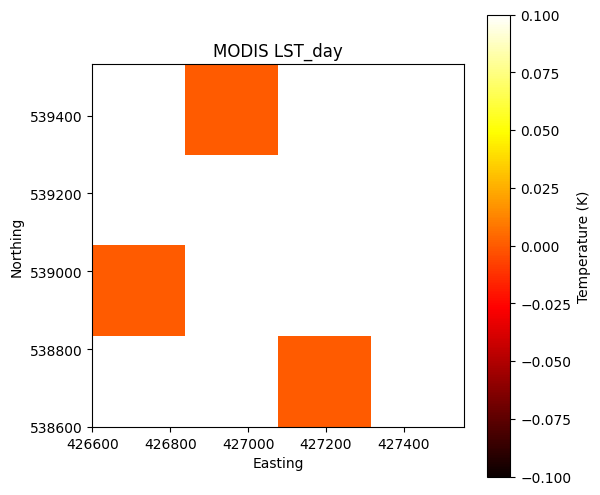
\includegraphics[width=0.5\textwidth]{modis_lst_day.png}
	\caption{MODIS LST Day}
	\label{fig:modis_day}
\end{figure}

\begin{figure}[H]
	\centering
	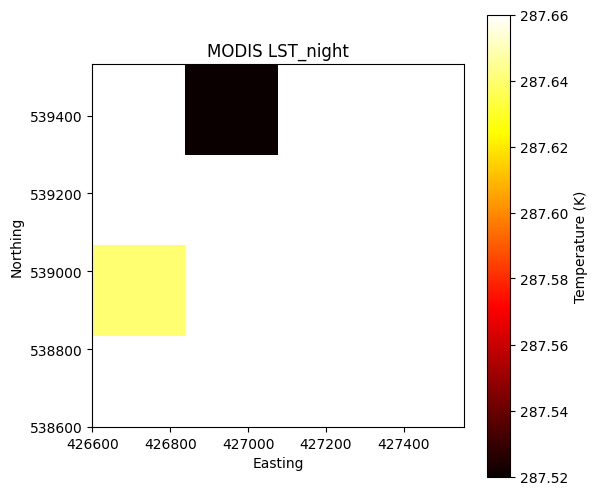
\includegraphics[width=0.5\textwidth]{modis_lst_night.png}
	\caption{MODIS LST Night}
	\label{fig:modis_night}
\end{figure}

\subsection{Data Integration}

The processed resistivity, GPR, satellite, and MODIS layers were combined into a single xarray Dataset object. This represents the datacube, with dimensions of easting, northing, and depth/layer as appropriate for each data type.

\section{Visualization}

The datacube layers were visualized as a 2D composite image using matplotlib (see Figure \ref{fig:composite}). The satellite imagery forms the base layer, with MODIS LST day values overlaid using a colormap and transparency. The resistivity models and GPR interpretation points are plotted at their respective locations.

\begin{figure}[H]
	\centering
	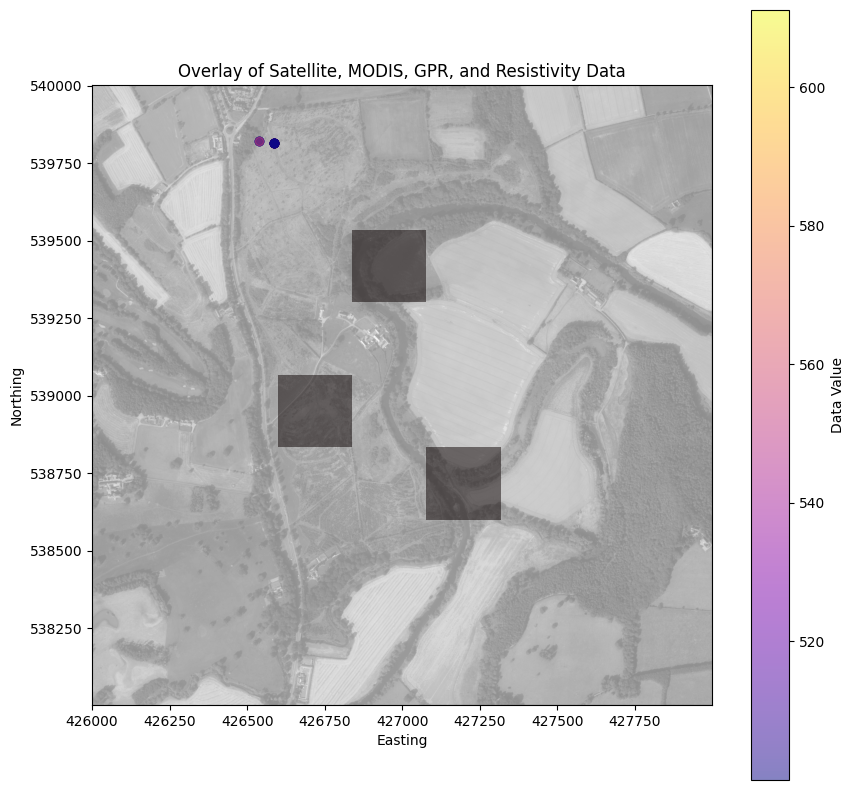
\includegraphics[width=0.7\textwidth]{datacube_composite.png}
	\caption{Composite 2D image of the data layers.}
	\label{fig:composite}
\end{figure}

A 3D interactive plot was attempted using plotly, but the large size of the dataset caused memory issues. (see Figure \ref{fig:3d})

\begin{figure}[H]
	\centering
	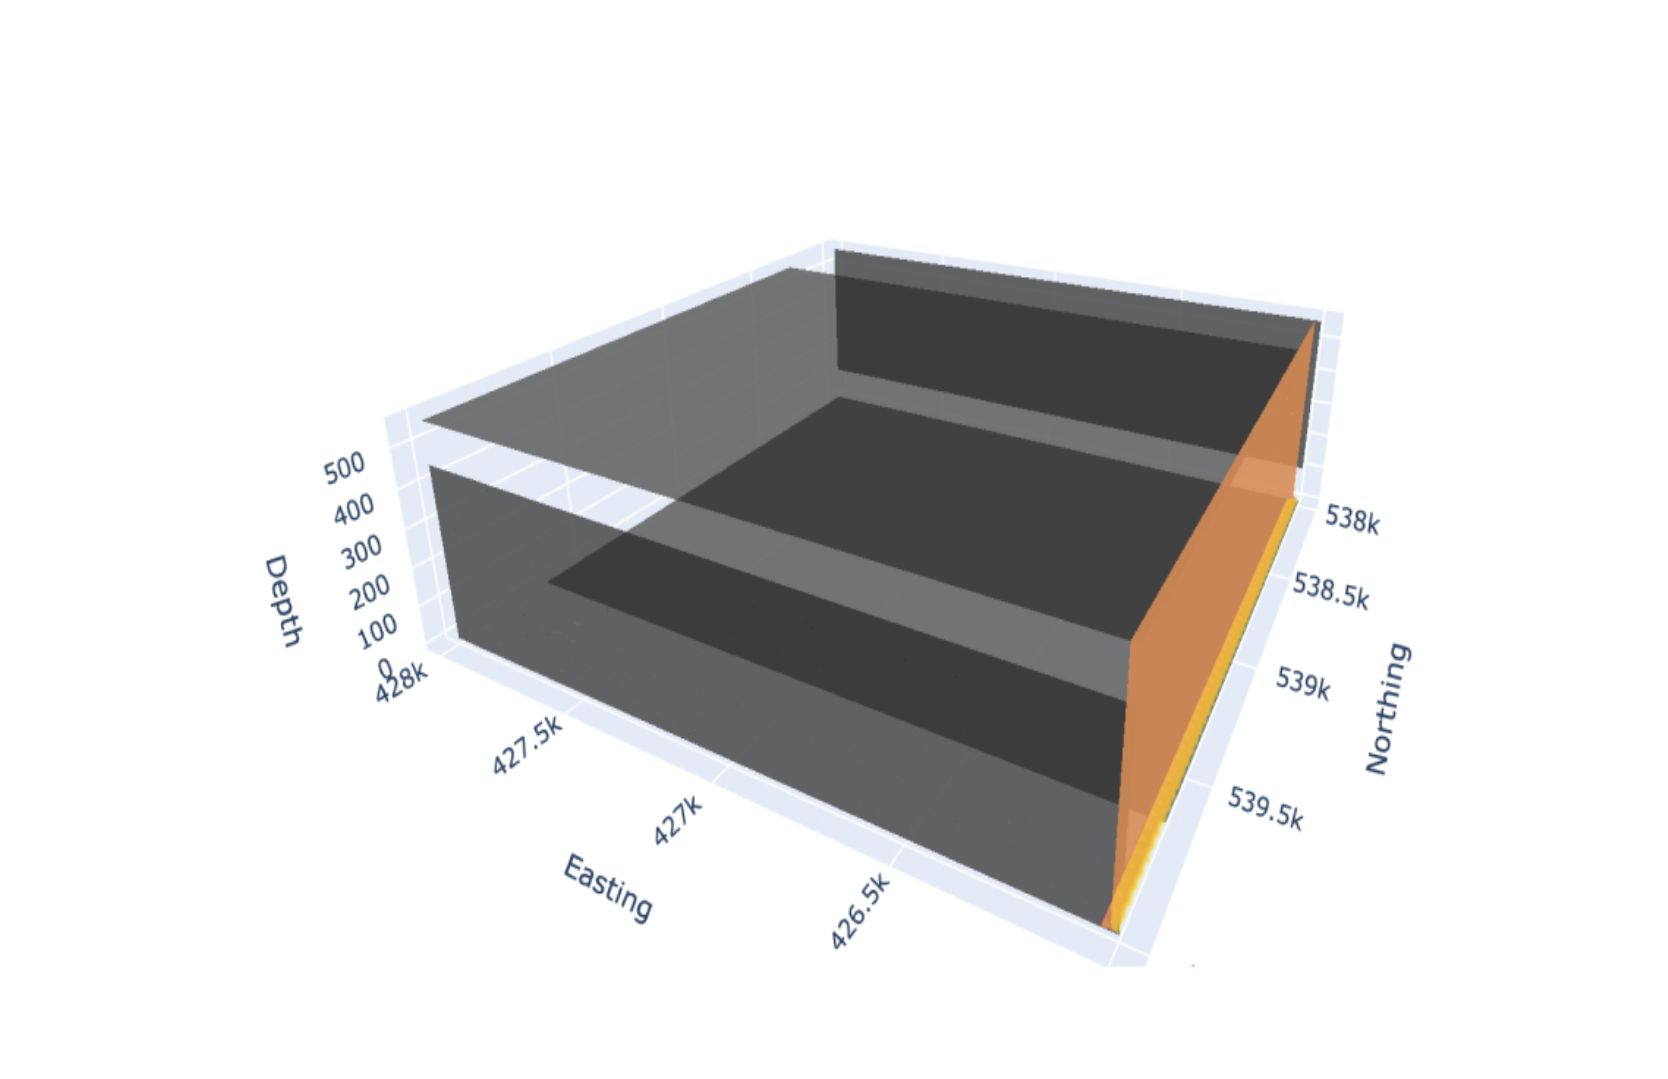
\includegraphics[width=0.63\textwidth]{faulty_3d.png}
	\caption{Faulty 3D image}
	\label{fig:3d}
\end{figure}

\section{Discussion}

\subsection{Achievements}

Despite the challenges encountered, the project achieved a successful integration of field measurements, satellite imagery and modelled data products into a 2D datacube structure. This required careful data cleaning, re-formatting and spatial alignment. The resulting 2D composite visualization provides an informative overview of the spatial patterns and interrelationships of surface and subsurface properties across the Low Burn Hall Estate.

The combination of inversions of field data (resistivity), direct measurements (GPR), remotely sensed imagery and modelled products (MODIS) leverages their strengths. The 2D image communicates a comprehensive characterization of the site that would be difficult to determine from any individual data source.

\subsection{Challenges and Limitations}

The lack of spatial reference information for the GPR and resistivity data was a significant challenge. The manual assignment of these data to approximate locations based on survey notes introduces potential inaccuracies in the integrated product. Improved field data collection practices that include recording GPS locations at each measurement site would improve data integration and enhance the reliability of the datacube.

The computational demands of processing and visualizing the large, multi-dimensional dataset posed difficulties. In particular, memory constraints prevented the realization of the planned interactive 3D datacube visualization. This limitation could potentially be overcome by employing cloud computing resources or high-performance computing infrastructure to handle the intensive data processing and rendering.

The MODIS data products, while useful for capturing broad landscape patterns, have a coarse spatial resolution of 1 km. This limits their utility for characterizing finer-scale spatial characterization within the estate. Incorporation of higher resolution remotely sensed data (e.g., Landsat, Sentinel) could provide more detailed insights.

\subsection{Future Directions}

Following methods could be taken to enhance the datacube and its derived products.

\begin{itemize}
	\item Improved field data collection protocols that include GPS locations for all measurements
	\item Leveraging high-performance computing resources to enable 3D interactive datacube visualization
	\item Incorporation of higher resolution remotely sensed data products
	\item Application of advanced machine learning algorithms (e.g., Deep Learning) for data fusion and pattern extraction
	\item Development of a web-based interface for easy access to and interaction with the datacube
	\item Adoption of the Open Data Cube framework for enhanced data management and analysis
\end{itemize}

The Open Data Cube (ODC) framework is a powerful tool for managing and analysing large volumes of geospatial data. It provides a set of APIs and tools for indexing, querying and processing data stored in a datacube format. The ODC framework offers several advantages that could significantly enhance the Low Burn Hall Estate datacube.

\begin{itemize}
	\item \textbf{Scalability}: The ODC framework is designed to handle PB-scale datasets, making it well-suited for managing the growing volume of data collected at the estate.
	\item \textbf{Interoperability}: The framework supports a wide range of data formats and sources, facilitating the integration of diverse datasets into a unified datacube.
	\item \textbf{Analysis-ready data}: ODC provides tools for preprocessing and standardizing data, ensuring that it is analysis-ready and consistent across time and space.
	\item \textbf{Efficient data access}: The indexing and querying capabilities enable rapid extraction of relevant subsets of data for analysis.
	\item \textbf{Collaborative development}: ODC is an open-source project with a growing community of developers and users, providing opportunities for collaboration and continuous improvement of the platform.
\end{itemize}

\section{Conclusion}

The integration of multi-source spatial data for the Low Burn Hall Estate shows the potential of datacubes for comprehensive environmental characterization. By combining field measurements, remotely sensed imagery and modelled data products, we can gain a general understanding of the interrelationships between surface and subsurface properties.

The key challenges encountered in this project - particularly the lack of spatial reference information for field data and the computational demands of large, multi-dimensional datasets - highlight areas for methodological improvement. Future work should prioritize the collection of GPS locations for all field measurements and the utilization of high-performance computing resources for data processing and visualization.

\section{GitHub Repository}

The code and datasets used in this project are available in the following GitHub repository: \href{https://github.com/suddenBook/DU-EE-Term_2-Datacube}{DU-EE-Term\_2-Datacube}.

\end{document}